\section{Operation Modes of Bipolar Junction Transistor}

\subsection{Experiment Design}
    \subsubsection{Background}
    There are two types of Bipolar Junction Transistors: NPN type and PNP types. They are difference in structure and have a symetric response to the circuit enviroment.\par

    In this experiment, we are going to learn operation modes of both type of BJT.\par

    \subsubsection{Propose}
    \begin{itemize}
        \item To test the different operation modes of a npn BJT
        \item To test the different operation modes of a pnp BJT
    \end{itemize}

\subsection{Experiment Design}
    \subsubsection{Materials}
        In this experiment, we will use the following components:
        \begin{itemize}
            \item 2N3904\_1 BJT (NPN)
            \item 2N3906\_1 BJT (PNP)
            \item Resistors
            \item Breadboard
            \item DC power supply
            \item Digital Multi-Meter
        \end{itemize}

    \subsubsection{Circuit Diagram}
        The following circuit diagrams 
        \begin{figure}[H]
            \centering
            \begin{subfigure}{0.4\textwidth}
                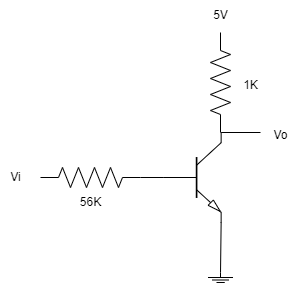
\includegraphics[width=1\linewidth]{Experiment_05/Circuits/Lab5a.png}
                \caption{Circuit for NPN BJT}
                \label{cir:5NPN}
            \end{subfigure}
            \begin{subfigure}{0.4\textwidth}
                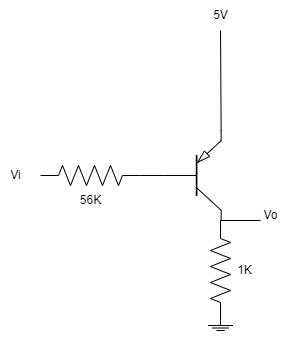
\includegraphics[width=1\linewidth]{Experiment_05/Circuits/Lab5b.png}
                \caption{Circuit for PNP BJT}
                \label{cir:5PNP}
            \end{subfigure}
            \caption{Minimal working Circuit for NPN and PNP BJT}
        \end{figure}

    \subsubsection{Theoretical Analysis}
        \begin{enumerate}[a]
            \item \textbf{The NPN BJT}\par
                NPN BJT have one P-type semi-conductor between two layers of N-type semi-conductor, and therefore it work in forward-biased when the base is positive.\par 
                Because of the symetric of two types of BJT, the NPN BJT will work in the opposite way of the PNP BJT, and here we will analyze the circuit of NPN BJT in figure \ref{cir:5NPN}.\par
        
                The $I_B$ can we express by KVL:
                \begin{equation}
                    I_B =
                        \begin{cases} 
                            0, & V_i < 0.6 \, \text{V} \, \text{(cutoff)} \\ 
                            \frac{V_i - 0.6}{R_B}, & V_i \geq 0.6 \, \text{V} \, \text{(active or saturation)}
                        \end{cases}
                \end{equation}
        
                Then, we can calculate the collector current
                \begin{equation}
                    I_C =
                    \begin{cases}
                        0, & \text{cutoff region} \\ 
                        \beta I_B, & \text{forward-active region (unsaturated)}
                    \end{cases}
                \end{equation}
        
                The output voltage can be calculated as 
                \begin{equation}
                    V_o =
                    \begin{cases}
                        5 \, \text{V}, & V_i < 0.6 \, \text{V} \\ 
                        5 \, \text{V} - I_C R_C, & 0.6 \, \text{V} < V_i < 1.944 \, \text{V} \\ 
                        V_{CE,\text{sat}} \approx 0.2 \, \text{V}, & V_i \geq 1.944 \, \text{V}
                    \end{cases}
                \end{equation}
        
            \item \textbf{The PNP BJT}\par
                PNP BJT have one N-type semi-conductor between two layers of P-type semi-conductor, and therefore it work in forward-biased when the base is negative.\par

                For the PNP BJT, the operation modes are the same as the NPN BJT, but the direction of the current and voltage are opposite, which is:
                \begin{equation}
                    V_o =
                        \begin{cases}
                            0, & V_i > 4.4 \, \text{V} \\ 
                            I_C R_C, & 3.056 \, \text{V} < V_i \leq 4.4 \, \text{V} \\ 
                            5 - V_{CE,\text{sat}} \approx 4.8 \, \text{V}, & V_i \leq 3.056 \, \text{V}
                        \end{cases}
                \end{equation}
        
        \end{enumerate}


\subsection{Experiment record}
    \subsubsection{NPN BJT}
    \begin{enumerate}[I]
        \item \textbf{Data Recorded}\newline
            The recorded data for the integration operation circuit is shown in the following table:
            \begin{table}[H]
                \centering
                \begin{tabular}{|c|c|c|c|c|c|c|c|c|c|}
                    \hline
                    Vi   & 0    & 0.25 & 0.5   & 0.6   & 0.75  & 0.82  & 1     & 1.5   & 1.6   \\ \hline
                    Vo   & 4.91 & 4.91 & 4.91  & 4.78  & 4.22  & 3.85  & 2.25  & 0.24  & 0.24  \\ \hline
                    Theo & 5    & 5    & 5     & 5     & 4.46  & 4.21  & 3.57  & 0.2   & 0.2   \\ \hline
                    Vi   & 1.65 & 1.7  & 1.75  & 1.8   & 1.9   & 2     & 3     & 4     & 5     \\ \hline
                    Vo   & 0.21 & 0.2  & 0.191 & 0.181 & 0.171 & 0.163 & 0.123 & 0.106 & 0.095 \\ \hline
                    Theo & 0.2  & 0.2  & 0.2   & 0.2   & 0.2   & 0.2   & 0.2     & 0.2     & 0.2     \\ \hline
                \end{tabular}
                \caption{Recorded Data for NPN BJT}
                \label{tab:}
            \end{table}
        \item \textbf{Data Analysis}\newline
            The expected output voltage is calculate using the theoretical analysis, and the result is shown in the table above. From the table we can see that the output voltage is close to the theoretical value, so our experiment is successful.
    \end{enumerate}

    \subsubsection{PNP BJT}
    \begin{enumerate}[I]
        \item \textbf{Data Recorded}\newline
            The recorded data for the integration operation circuit is shown in the following table:
            \begin{table}[H]
                \centering
                \begin{tabular}{|c|c|c|c|c|c|c|c|c|c|}
                    \hline
                    Vi   & 0    & 0.65 & 1.41 & 2.09 & 2.48 & 2.98  & 3.13  & 3.26 & 3.48 \\ \hline
                    Vo   & 4.83 & 4.82 & 4.81 & 4.79 & 4.77 & 4.8  & 4.09  & 3.69 & 3    \\ \hline
                    Theo & 4.8  & 4.8  & 4.8  & 4.8  & 4.8  & 5.10  & 4.56  & 4.09 & 3.30 \\ \hline
                    Vi   & 3.61 & 3.76 & 3.92 & 4.06 & 4.19 & 4.21  & 4.49  & 5    &      \\ \hline
                    Vo   & 2.55 & 2.04 & 1.5  & 1.03 & 0.65 & 0.587 & 0.004 & 0    &      \\ \hline
                    Theo & 2.84 & 2.30 & 1.72 & 1.22 & 0.75 & 0.68  & 0     & 0    &      \\ \hline
                \end{tabular}
                \caption{Recorded Data for PNP BJT}
                \label{tab:}
            \end{table}
        \item \textbf{Data Analysis}\newline
            The expected output voltage is calculate using the theoretical analysis, and the result is shown in the table above. From the table we can see that the output voltage is close to the theoretical value, so our experiment is successful.
    \end{enumerate}
    
\subsection{Experiment Conclusion}
    \subsubsection{Conclusion}
    In this experiment, we have learned the operation modes of both NPN and PNP BJT. We have tested the circuit of both type of BJT, and observe the citcuit behaive in three different operation mode.